\documentclass[12pt]{report}
\usepackage[utf8]{inputenc}
\usepackage[russian]{babel}
%\usepackage[14pt]{extsizes}
\usepackage{listings}

\usepackage{graphicx}
\graphicspath{{src/}}
\DeclareGraphicsExtensions{.pdf,.png,.jpg}

\usepackage{amsmath,amsfonts,amssymb,amsthm} 

% Для листинга кода:
\lstset{ %
language=c++,                 % выбор языка для подсветки (здесь это С++)
basicstyle=\small\sffamily, % размер и начертание шрифта для подсветки кода
numbers=left,               % где поставить нумерацию строк (слева\справа)
numberstyle=\tiny,           % размер шрифта для номеров строк
stepnumber=1,                   % размер шага между двумя номерами строк
numbersep=5pt,                % как далеко отстоят номера строк от подсвечиваемого кода
showspaces=false,            % показывать или нет пробелы специальными отступами
showstringspaces=false,      % показывать или нет пробелы в строках
showtabs=false,             % показывать или нет табуляцию в строках
frame=single,              % рисовать рамку вокруг кода
tabsize=2,                 % размер табуляции по умолчанию равен 2 пробелам
captionpos=t,              % позиция заголовка вверху [t] или внизу [b] 
breaklines=true,           % автоматически переносить строки (да\нет)
breakatwhitespace=false, % переносить строки только если есть пробел
escapeinside={\#*}{*)}   % если нужно добавить комментарии в коде
}

% Для измененных титулов глав:
\usepackage{titlesec, blindtext, color} % подключаем нужные пакеты
\definecolor{gray75}{gray}{0.75} % определяем цвет
\newcommand{\hsp}{\hspace{20pt}} % длина линии в 20pt
% titleformat определяет стиль
\titleformat{\chapter}[hang]{\Huge\bfseries}{\thechapter\hsp\textcolor{gray75}{|}\hsp}{0pt}{\Huge\bfseries}


% plot
\usepackage{pgfplots}
\usepackage{filecontents}
\usetikzlibrary{datavisualization}
\usetikzlibrary{datavisualization.formats.functions}


\begin{document}
\begin{titlepage}
	\centering
	{\scshape\LARGE МГТУ им. Баумана \par}
	\vspace{3cm}
	{\scshape\Large Лабораторная работа №6\par}
	\vspace{0.5cm}	
	{\scshape\Large По курсу: "Анализ алгоритмов"\par}
	\vspace{1.5cm}
	{\huge\bfseriesМуравьиный алгоритм\par}
	\vspace{2cm}
	\Large Работу выполнила: Оберган Татьяна, ИУ7-55Б\par
	\vspace{0.5cm}
	\LargeПреподаватели:  Волкова Л.Л., Строганов Ю.В.\par

	\vfill
	\large \textit {Москва, 2019} \par
\end{titlepage}

\tableofcontents

\newpage
\chapter*{Введение}
\addcontentsline{toc}{chapter}{Введение}
Муравьиный алгоритм — один из эффективных полиномиальных алгоритмов для нахождения приближённых решений задачи коммивояжёра, а также решения аналогичных задач поиска маршрутов на графах.
        
Целью данной лабораторной работы является изучение муравьиных алгоритмов и приобретение навыков параметризации методов на примере муравьиного алгоритма, примененного к задаче коммивояжера.
        
Задачи данной лабораторной работы:
\begin{itemize}
	\item рассмотренть муравьиный алгоритм и алгоритм полного перебора в задаче коммивояжера;
	\item реализовать эти алгоритмы;
	\item сравнить время работы этих алгоритмов.
\end{itemize}



\chapter{Аналитическая часть}
В данной части будут рассмотрены теоретические основы задачи коммивояжера и муравьиного алгоритма. 
		
\section{Постановка задачи} 
Имеется сильно связный взвешенный ориентированный граф \cite{diskr} с положительными весами, заданный в виде матрицы смежностей. Количество вершин в нем лежит в диапазоне от 5 до 20.Требуется решить задачу коммивояжера для этого графа. 
\section{Задача коммивояжера}
 Коммивояжёр (фр. commis voyageur) — бродячий торговец. Задача коммивояжёра — важная задача транспортной логистики, отрасли, занимающейся планированием транспортных перевозок. Коммивояжёру, чтобы распродать нужные и не очень нужные в хозяйстве товары, следует объехать n пунктов и в конце концов вернуться в исходный пункт. Требуется определить наиболее выгодный маршрут объезда. В качестве меры выгодности маршрута (точнее говоря, невыгодности) может служить суммарное время в пути, суммарная стоимость дороги, или, в простейшем случае, длина маршрута \cite{commi2}.

\section{Решение полным перебором}
Задача может быть решена перебором всех вариантов объезда и выбором оптимального. Но при таком подходе количество возможных маршрутов очень быстро возрастает с ростом n (оно равно n! — количеству способов упорядочения пунктов). К примеру, для 100 пунктов количество вариантов будет представляться 158-значным числом — не выдержит ни один калькулятор! Мощная ЭВМ, способная перебирать миллион вариантов в секунду, будет биться с задачей на протяжении примерно 3*10144 лет. Увеличение производительности ЭВМ в 1000 раз даст хоть и меньшее в 1000 раз, но по-прежнему чудовищное время перебора вариантов. Не спасает ситуацию даже то, что для каждого варианта маршрута имеется 2n равноценных, отличающихся выбором начального пункта (n вариантов) и направлением обхода (2 варианта). Перебор с учётом этого наблюдения сокращается незначительно \cite{commi}. % до $\frac{n!}{2n}=\frac{(n−1)!}{2}$ вариантов \cite{commi}.	
\section{Муравьиные алгоритмы}
Все муравьиные алгоритмы базируются на моделировании поведения колонии муравьев. Колония муравьев может рассматриваться как многоагентная система, в которой каждый агент (муравей) функционирует автономнопо очень простым правилам. В противовес почтипримитивному поведению агентов, поведениевсей системы получается на удивление разумным.
		
Муравьиные алгоритмы представляют собой вероятностную жадную эвристику, где вероятности устанавливаются, исходя из информации о качестве решения, полученной из предыдущих решений.

Идея муравьиного алгоритма - моделирование поведения муравьёв, связанного с их способностью быстро находить кратчайший путь от муравейника к источнику пищи и адаптироваться к изменяющимся условиям, находя новый кратчайший путь\cite{ant1}. При своём движении муравей метит путь феромоном, и эта информация используется другими муравьями для выбора пути. Это элементарное правило поведения и определяет способность муравьёв находить новый путь, если старый оказывается недоступным.

Какие же механизмы обеспечивают столь сложное поведение муравьев, и что можем мыпозаимствовать у этих крошечных существ длярешения своих глобальных задач? Основу «социального» поведения муравьев составляет самоорганизация — множество динамических механизмов, обеспечивающих достижение системой глобальной цели в результате низкоуровневого взаимодействия ее элементов. Принципиальнойособенностью такого взаимодействия являетсяиспользование элементами системы только локальной информации. При этом исключается любое централизованное управление и обращениек глобальному образу, репрезентирующему систему во внешнем мире. Самоорганизация является результатом взаимодействия следующих четырех компонентов \cite{shtovba} :
	\begin{itemize}
	\item случайность;
	\item многократность;
	\item положительная обратная связь;
	\item отрицательная обратная связь.
	\end{itemize}

Рассмотрим случай, когда на оптимальном доселе пути возникает преграда. В этом случае необходимо определение нового оптимального пути. Дойдя до преграды, муравьи с равной вероятностью будут обходить её справа и слева. То же самое будет происходить и на обратной стороне преграды. Однако, те муравьи, которые случайно выберут кратчайший путь, будут быстрее его проходить, и за несколько передвижений он будет более обогащён феромоном. Поскольку движение муравьёв определяется концентрацией феромона, то следующие будут предпочитать именно этот путь, продолжая обогащать его феромоном до тех пор, пока этот путь по какой-либо причине не станет недоступен.

Очевидная положительная обратная связь быстро приведёт к тому, что кратчайший путь станет единственным маршрутом движения большинства муравьёв. Моделирование испарения феромона - отрицательной обратной связи - гарантирует нам, что найденное локально оптимальное решение не будет единственным - муравьи будут искать и другие пути. Если мы моделируем процесс такого поведения на некотором графе, рёбра которого представляют собой возможные пути перемещения муравьёв, в течение определённого времени, то наиболее обогащённый феромоном путь по рёбрам этого графа и будет являться решением задачи, полученным с помощью муравьиного алгоритма.

Обобщим все выше сказанное. Любой муравьиный алгоритм, независимо от модификаций, представим в следующем виде:
\begin{itemize}
	\item Создание муравьев;
	\item Поиск решения;
	\item Обновление феромона;
	\item Дополнительные действия (опиционально).
\end{itemize}

Теперь рассмотрим каждый шаг в цикле более подробно:\\

1. Создание муравьев\\
   Стартовая точка, куда помещается муравей, зависит ограничений,   накладываемых условиями задачи. Потому что для каждой задачи   способ размещения муравьёв является определяющим. Либо все    они помещаются в одну точку, либо в разные с повторения, либо    без повторений. \\
  На этом же этапе задается начальный уровень феромона. Он    инициализируется небольшим положительным числом для того,    чтобы на начальном шаге вероятности перехода в следующую    вершину не были нулевыми. \\
  
2. Поиск решения  \\
 Вероятность перехода из вершины i в вершину j определяется по следующей формуле\ref{form:way}\\   
\begin{equation}\label{form:way} 
 p_{i,j}={\frac {(\tau _{i,j}^{\alpha })(\eta _{i,j}^{\beta })}{\sum (\tau _{i,j}^{\alpha })(\eta _{i,j}^{\beta })}}
 \end{equation}
    где \quad$ \tau _{i,j} - $ расстояние от города i до j;
    
         $\eta _{i,j} - $количество феромонов на ребре ij;
         
          $\alpha - $ параметр влияния длины пути;
          
          $\beta - $ параметр влияния феромона.


3. Обновление феромона \\
  Уровень феромона обновляется в соответствии с приведённой формулой:\\
После того, как муравей успешно проходит маршрут, он оставляет на всех пройденных ребрах след, обратно пропорциональный длине пройденного пути. Итого, новый след феромона вычисляется по формуле \ref{form:eva}:
\begin{equation}\label{form:eva} 
    \tau _{i,j}=(1-\rho )\tau _{i,j}+\Delta \tau _{i,j},
\end{equation}
где \quad$ \rho _{i,j}$ - \text{доля феромона, который испарится;} 

    $\tau _{i,j}$ - \text{количество феромона на дуге ij;} 
    
    $\Delta \tau _{i,j}$ - \text{количество отложенного феромона, вычисляется по формуле \ref{form:add1}.}

4. Дополнительные действия 

 Обычно здесь используется алгоритм локального поиска, однако    он может также появиться и после поиска всех решений. 

\section{Муравьиный алгоритм в задаче коммивояжера}
Рассмотрим, как реализовать четыре составляющие самоорганизации муравьев при оптимизации маршрута коммивояжера. Многократность взаимодействия реализуется итерационным поиском маршрута коммивояжера одновременно несколькими муравьями. При этом каждый муравей рассматривается как отдельный, независимыйкоммивояжер, решающий свою задачу. За однуитерацию алгоритма каждый муравей совершаетполный маршрут коммивояжера.Положительная обратная связь реализуется как имитация поведения муравьев типа «оставление следов – перемещение по следам». Чем больше следов оставлено на тропе — ребре графа в задаче коммивояжера, тем больше муравьев будет передвигаться по ней. При этом на тропе появляются новые следы, привлекающие дополнительных муравьев. Для задачи коммивояжера положительная обратная связь реализуется следующим стохастическим правилом: вероятность включения ребра графа в маршрут муравья пропорциональна количеству феромона на нем.
		
Теперь с учетом особенностей задачи коммивояжёра, мы можем описать локальные правила поведения муравьев при выборе пути.\
		
	1. Муравьи имеют собственную «память». Поскольку каждый город может быть посещён только один раз, то у каждого муравья есть список уже посещенных городов - список запретов. Обозначим через $J$ список городов, которые необходимо посетить муравью $k$ , находящемуся в городе $i$ . 
	
	2. Муравьи обладают «зрением» - видимость есть эвристическое желание посетить город $j$ , если муравей находится в городе $i$ . Будем считать, что видимость обратно пропорциональна расстоянию между городами. 
	
	3. Муравьи обладают «обонянием» - они могут улавливать след феромона, подтверждающий желание посетить город $j$ из города $i$ на основании опыта других муравьёв. Количество феромона на ребре $(i,j)$ в момент времени $t$ обозначим через  $tau _{i,j} (t)$ 
	
	 4. На этом основании мы можем сформулировать вероятностнопропорциональное правило, определяющее вероятность перехода $k$-ого муравья из города $i$  в город $j$. 
	 
	5. Пройдя ребро $(i,j)$ , муравей откладывает на нём некоторое количество феромона, которое должно быть связано с оптимальностью сделанного выбора. Пусть $T _{k} (t)$ есть маршрут, пройденный муравьем $k$ к моменту времени $t$ , $L _{k} (t)$ - длина этого маршрута, а $Q$ - параметр, имеющий значение порядка длины оптимального пути. Тогда откладываемое количество феромона может быть задано в виде:
	
 \begin{equation}\label{form:add} 
    {\displaystyle \Delta \tau _{i,j}^k={\begin{cases}Q/L_{k}& {\mbox{Если k-ый мурваей прошел по ребру ij;}}\\0&{\mbox{Иначе}}\end{cases}}}
\end{equation}
   где \quad Q - количество феромона, переносимого муравьем;
   
 Тогда
 \begin{equation}\label{form:add1} 
    \Delta \tau _{i,j}= \tau _{i,j}^0 + \tau _{i,j}^1 + ... + \tau _{i,j}^k 
\end{equation}
   
    где k - количество муравьев в вершине графа с индексами i и j.

	
\section*{Вывод}
\addcontentsline{toc}{section}{Введение}
В данном разделе были рассмотрены общие принципы муравьиного алгоритма и применение его к задаче коммивояжера. 





\chapter{Конструкторская часть}
В данном разделе будут рассмотрены основные требования к программе и схемы алгоритмов.

\section{Требования к программе}
\textbf{Требования к вводу:}
у ориентированного графа должно быть хотя бы 2 вершины.
\newline
\textbf{Требования к программе:}
\begin{itemize}
\item алгоритм полного перебора должен возвращать кратчайший путь в графе.
\end{itemize}
 .  
\newline  
\textbf{Входные данные} - матрица смежности графа.  
\newline
\textbf{Выходные данные} - самый выгодный путь.

\section{Схемы алгоритмов}
На рисунке 2.1 и 2.2 приведены схемы алгоритмов решения задачи коммивояжера.\\

\newpage
\begin{figure}[h]
        	\center{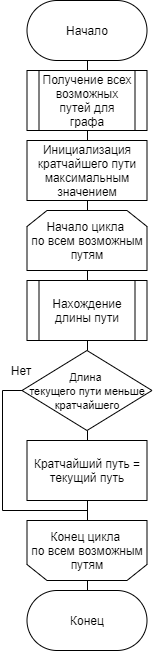
\includegraphics[scale = 0.5]{BruteForce.png}}
        	\caption{Схема алгоритма полного перебора}
        	\label{fig:f_p}
\end{figure}
        \newpage   

\begin{figure}[h]
        	\center{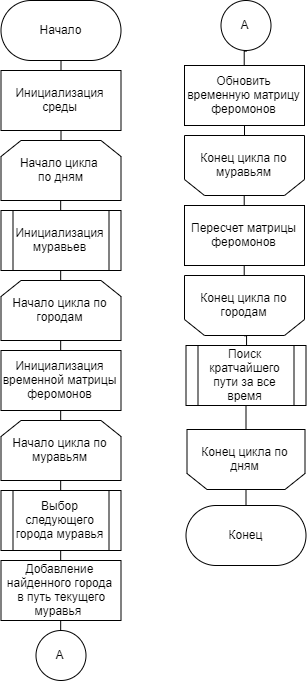
\includegraphics[scale = 0.5]{Ant.png}}
        	\caption{Схема муравьиного агоритма}
        	\label{fig:ant}
\end{figure}
\newpage

\section*{Вывод}
\addcontentsline{toc}{section}{Вывод}
В данном разделе были рассмотрены требования к программе и схемы алгоритмов.


 

\chapter{Технологическая часть}
Замеры времени были произведены на: Intel(R) Core(TM) i5-8300H, 4 ядра, 8 логических процессоров.

\section{Выбор ЯП}
В качестве языка программирования был выбран C\# \cite{Microsoft}. Средой разработки Visual Studio. 
Время работы алгоритмов было замерено с помощью класса Stopwatch. 

\section{Сведения о модулях программы}
Программа состоит из:
\begin{itemize}
	\item Program.cs - главный файл программы, в котором располагается точка входа в программу
	\item BruteForce.cs - функции полного перебора
	\item AntAlgorithm.cs - функция муравьиного алгоритма и дополнительные классы для этого алгоритма
\end{itemize}


\section{Листинг кода алгоритмов}
В этой части будут рассмотрены листинги кода (листинг 3.1 - 3.3) реализованых алгоритмов.
\begin{lstlisting}[label=some-code,caption=Алгоритм поиска полным перебором]
public static Path GetShortestPath(Map m)
        {
            int[] routeIndexes = new int[m.n - 1];
            for (int i = 0; i < m.n - 1; i++)
            {
                routeIndexes[i] = i + 1;
            }
            var allRoutes = GetAllRoutes(routeIndexes);
            Path shortestPath = new Path(int.MaxValue);
            foreach (List<int> path in allRoutes)
            {
                path.Insert(0, 0);
                path.Add(0);
                Path cur = new Path(m, path.ToArray());
                if (cur.distance < shortestPath.distance)
                    shortestPath = cur;
            }

            return shortestPath;
        }
\end{lstlisting}

\begin{lstlisting}[label=some-code,caption=Алгоритм поиска всех перестановок]
public static List<List<T>> GetAllRoutes<T>(IList<T> arr, List<List<T>> res = null, List<T> current = null)
        {
            if (res == null)
                res = new List<List<T>>();
            if (arr.Count == 0)
            {
                res.Add(current);
                return res;
            }
            for (int i = 0; i < arr.Count; i++)
            {
                List<T> lst = new List<T>(arr);
                lst.RemoveAt(i);
                List<T> next;
                if (current == null)
                    next = new List<T>();
                else
                    next = new List<T>(current);
                next.Add(arr[i]);
                GetAllRoutes(lst, res, next);
            }
            return res;
        }
\end{lstlisting}

\begin{lstlisting}[label=some-code,caption=Муравьиный алгоритм]
public static Path GetShortestPath(Map map, int nIter, double alpha, double beta, double Q, double ro)
        {
            Path minPath = new Path(int.MaxValue);
            int n = map.n;
            double[][] pheromones = Program.InitMatr(n, 0.1);

            List<Ant> ants = new List<Ant>();
            for (int t = 0; t < nIter; t++) // days
            {
                ants = InitAnts(map, n);

                // colony route
                for (int i = 0; i < n - 1; i++)
                {
                    double[][] pheromonesIter = Program.InitMatr(n, (double)0); // 1 colony step

                    for (int j = 0; j < ants.Count(); j++) // ants
                    {
                        double sumChance = 0, chance = 0;
                        bool flag = false;
                        Ant curAnt = ants[j];
                        int curCity = curAnt.path.route.Last();
                        for (int sityId = 0; sityId < n; sityId++) 
                        {
                            if (curAnt.visited[sityId] == false)
                            {
                                sumChance += Math.Pow(pheromones[curCity][sityId], alpha) * Math.Pow(1 / (map.distance[curCity][sityId]), beta);
                                flag = true;
                            }
                        }
                        double x = r.NextDouble();
                        int k = 0;
                        for (; x > 0; k++)
                        {
                            if (curAnt.visited[k] == false)
                            {
                                chance = Math.Pow(pheromones[curCity][k], alpha) * Math.Pow(1 / (map.distance[curCity][k]), beta);
                                chance /= sumChance;
                                x -= chance;
                            }
                        }
                        k--;
                        ants[j].VisitedTown(k);
                        pheromonesIter[curCity][k] += Q / (map.distance[curCity][k]);
                    }

                    for (int ii = 0; ii < n; ii++)
                        for (int j = 0; j < n; j++)
                            pheromones[ii][j] = (1 - ro) * pheromones[ii][j] + pheromonesIter[ii][j];
                }
                
                foreach (Ant a in ants)
                {
                    a.VisitedTown(a.iStartTown);
                    if (a.GetDistance() < minPath.distance)
                    {
                        minPath = a.path;
                    }
                }                
            }
            return minPath;
        }
\end{lstlisting}

\section*{Вывод}
\addcontentsline{toc}{section}{Вывод}
В данном разделе были рассмотрены основные сведения о модулях программы и листинг кода алгоритмов.




\chapter{Исследовательская часть}
В даннном разделе будет проведен сравнительный временной анализ алгоритмов и рассмотрена параметризация муравьиного алгоритма.

\section{Сравнительный анализ на основе замеров времени}
Был проведен замер времени работы алгоритмов при разных размерах графа. На рис.4.1 и рис.4.2 показаны результаты замеров времени.


\begin{tikzpicture}
\begin{axis}[
    	axis lines = left,
    	xlabel = {Количество вершин},
    	ylabel = {Время (тики)},
	legend pos=north west,
	ymajorgrids=true
]


\addplot[color=blue] table[x index=0, y index= 1] {Brute.txt}; 
\addlegendentry{Полный перебор}

\addplot[color=orange] table[x index=0, y index= 1] {Ant.txt}; 
\addlegendentry{Муравьиный алгоритм}


\end{axis}
\end{tikzpicture}
\begin{center}
Pис. 4.1: Сравнение времени работы алгоритмов при увеличении размера графа.
\end{center}

\begin{tikzpicture}
\begin{axis}[
    	axis lines = left,
    	xlabel = {Количество вершин},
    	ylabel = {Время (тики)},
	legend pos=north west,
	ymajorgrids=true
]


\addplot[color=blue] table[x index=0, y index= 1] {Brute2.txt}; 
\addlegendentry{Полный перебор}

\addplot[color=orange] table[x index=0, y index= 1] {Ant2.txt}; 
\addlegendentry{Муравьиный алгоритм}


\end{axis}
\end{tikzpicture}
\begin{center}
Pис. 4.2: Сравнение времени работы алгоритмов на малых размерах графа.
\end{center}

На рисунках 4.1 и 4.2 видно, что муравьиный алгоритм значительно выигрыает по скорости полному перебору при размере графа больше 9.
До 8 вершины алгоритм полного перебора работает быстрее, с максимальным выигрышем по времени в 2,5 раза, при 6 вершинах.
На графе размера 10 полный перебор работает в 30 раз медленнее. 

\section{Параметризация муравьиного алгоритма}	

Для различных значений параметров $\alpha$, $\beta$, $\rho$ и $t_{max}$ для каждой из нескольких матриц смежности с помощью муравьиного алгоритма и перебора была найдена некоторая длина маршрута. Далее выбраны наилучшие сочетания параметров муравьиного алгоритма на этих данных.\\
Параметр $\alpha$ менялся от 0 до 10, параметр $\rho$ менялся от 0.1 до 0.9, параметр $t_{max}$ менялся от 5 до 100.\\
Итого были выявлены оптимальные сочетания параметров (представлены в таблице 4.1):\\

\begin{table}
	\caption{Результаты решения задачи параметризации}
	\begin{center}
		
	\begin{tabular}{|c|c|c|c|}
		\hline
		$\alpha$ &$\beta$ & $\rho$ & $t_{max}$ \\\hline
		4&6&0.6&20\\
		6&4&0.3&40\\
		 1&9&0.7&50\\
		 6&4&0.9&70\\
		 3&7&0.6&80\\
		 6&4&0.25&90\\
		 \hline
	\end{tabular}
\end{center}
\end{table} 
\

\section*{Вывод}
\addcontentsline{toc}{section}{Вывод}
Сравнительный анализ по времени показал, что после на больших размерностях (размер графа больше 9) полный перебор крайне медленен относительно муравьиного алгоритма.



\chapter*{Заключение}
\addcontentsline{toc}{chapter}{Заключение}
В ходе лабораторной работы я изучила возможности применения и реализовала алгоритм полного перебора и муравьиный алгоритм. 

Временной анализ показал, что неэффективно использовать полный перебор на графе размера больше 10.

\addcontentsline{toc}{chapter}{Список литературы}
 \begin{thebibliography}{3}
\bibitem{Microsoft}
Руководство по языку C\#[Электронный ресурс], - режим доступа: https://docs.microsoft.com/ru-ru/dotnet/csharp/
\bibitem{UnitTests}
Основные сведения о модульных тестах [Электронный ресурс], - режим доступа: https://docs.microsoft.com/ru-ru/visualstudio/test/unit-test-basics?view=vs-2019
\bibitem{diskr} Белоусов А.И., Ткачев С.Б(2006). Дискретная математика, 4-е издание.
\bibitem{commi2} Т.М. Товстик, Е.В. Жукова - Алгоритм приближенного решения задачи коммивояжера.
\bibitem{commi} Задача коммивояжера[Электронный ресурс] - режим доступа http://mech.math.msu.su/~shvetz/54/inf/perl-problems/chCommisVoyageur.xhtml
\bibitem{ant1} Муравьиные алгоритмы[Электронный ресурс] - режим доступа http://www.machinelearning.ru/wiki/index.php?title=%D0%9C%D1%83%D1%80%D0%B0%D0%B2%D1%8C%D0%B8%D0%BD%D1%8B%D0%B5_%D0%B0%D0%BB%D0%B3%D0%BE%D1%80%D0%B8%D1%82%D0%BC%D1%8B
\bibitem{shtovba} Штовба С.Д. - Муравьиные алгоритмы.
\bibitem{Beloysov} И. В. Белоусов(2006), Матрицы и определители, учебное пособие по линейной алгебре, с. 1 - 16
\end{thebibliography}


\end{document}